\documentclass[12pt]{article}
    \usepackage[spanish, es-tabla]{babel}
    \usepackage[top=2cm, bottom=2cm,left=2cm, right=2cm]{geometry}
    \usepackage[utf8x]{inputenc}
    \usepackage{amsmath}
    \usepackage{enumerate}
    \usepackage{graphicx}
    \graphicspath{ {capturas/} }
    \usepackage{xcolor}
    \usepackage{hyperref}
    \hypersetup{
    colorlinks=false,
    linkbordercolor={white}
    }
    \usepackage{listings}
    \usepackage{parskip}
    \lstset{
        language=C++,
        basicstyle=\ttfamily\scriptsize,
        keywordstyle=\color{blue}\ttfamily,
        otherkeywords={WIDTH},
        keywords=[2]{__shared__},
        keywordstyle=[2]\color{orange}\ttfamily,
        stringstyle=\color{red}\ttfamily,
        commentstyle=\color{green}\ttfamily,
        breaklines=true,
    }
  

    \newcommand{\img}[1]{
    \noindent\makebox[\textwidth][c]{\includegraphics[width=1\textwidth,]{#1}}%
    }

    \begin{document}  
    \hypersetup{pageanchor=false}

    \begin{titlepage}
        \newcommand{\HRule}{\rule{\linewidth}{0.5mm}}
        \center
        \textsc{\LARGE Universidad de Granada}\\[1cm] 
        \textsc{\large Ingeniería Informática}\\[0.5cm] 
        \HRule \\[0.4cm]
        { \huge \bfseries Entrega 2 - Calculadora en LEX}\\[0.4cm]
        \HRule \\[1.5cm]
        \large\emph{Autor: }\textsc{Juan Carlos Ruiz García}\\
        {\large\emph{Asignatura: Modelos de Computación }}\\
        {\large\emph\today}\\[2cm]
        
\includegraphics[scale=1.0]{logo.png}\\[1cm]
        \vfill
    \end{titlepage}

    \hypersetup{pageanchor=true}
    \tableofcontents
    \clearpage

\section{Problema planteado}

El problema planteado, es el desarrollo de una \textbf{calculadora utilizando LEX} y apoyandonos en \textbf{estructuras de datos} desarrolladas en \textbf{C++}.

La calculadora podrá realizar operaciones con \textbf{enteros y reales}. Además unicamente permitirá llevar a cabo las operaciones de \textbf{suma, resta, multiplicación y división}.


\subsection{Estructura de datos utilizada}
Para el desarrollo de la calculadora, hemos utilizado la siguiente estructura de datos:
\begin{lstlisting}[frame=single]
    vector<double> variables;
    vector<bool> variablesU;
    list<double> valores;
    list<pair<char,int> > simbolos;
\end{lstlisting}

\subsubsection{variables \& variablesU}
En la calculadora podremos definir hasta \textbf{26 variables} para realizar operaciones con ellas, siendo estas de la \textbf{'a-z' en minúscula}.
\begin{itemize}
    \item \textbf{variables} : vector de doubles utilizado para almacenar los valores de las 26 posibles variables.
    \item \textbf{variablesU} : vector de boolean inicialmente los 26 a false, menos las variables con valor asignado que estarán a true.
\end{itemize}

\subsubsection{valores \& simbolos}
Son dos listas enlazas utilizadas para:
\begin{itemize}
    \item \textbf{valores} : contiene los números que forman la operación a realizar.
    \item \textbf{simbolos} : contiene los operadores que se van a aplicar a los números del vector valores junto con su prioridad. Dicha prioridad se calcula:
    \begin{itemize}
        \item Con parentesis {\scriptsize(a)}:
        \begin{itemize}
            \item '+' y '-' : como \textbf{numParentesis*3}
            \item '*' y '/' : como \textbf{numParentesis*4} \newline
            {\scriptsize (a) numParentesis inicialmente vale 0. Se incrementa en 1 cuando se encuentra '(' y se decrementa en 1 cuando se encuentra ')'}
        \end{itemize}
        \item Sin parentesis {\scriptsize(b)}:
        \begin{itemize}
            \item '+' y '-' : como \textbf{prioSumRes}
            \item '*' y '/' : como \textbf{prioMulDiv}\newline
            {\scriptsize (b) prioSumRes = 1; prioMulDiv = 2;}
        \end{itemize}
    \end{itemize}
\end{itemize}

\subsection{Funcionamiento}
En la \textbf{lista de valores} se van almacenando los números que se van encontrando en la operación de izquierda a derecha, al igual que en
la \textbf{lista de simbolos} se van guardando los operadores encontrados junto con su correspondiente prioridad, calculada como se explicó anteriormente.

Un ejemplo de funcionamiento sería el siguiente:

\noindent\makebox[\textwidth][c]{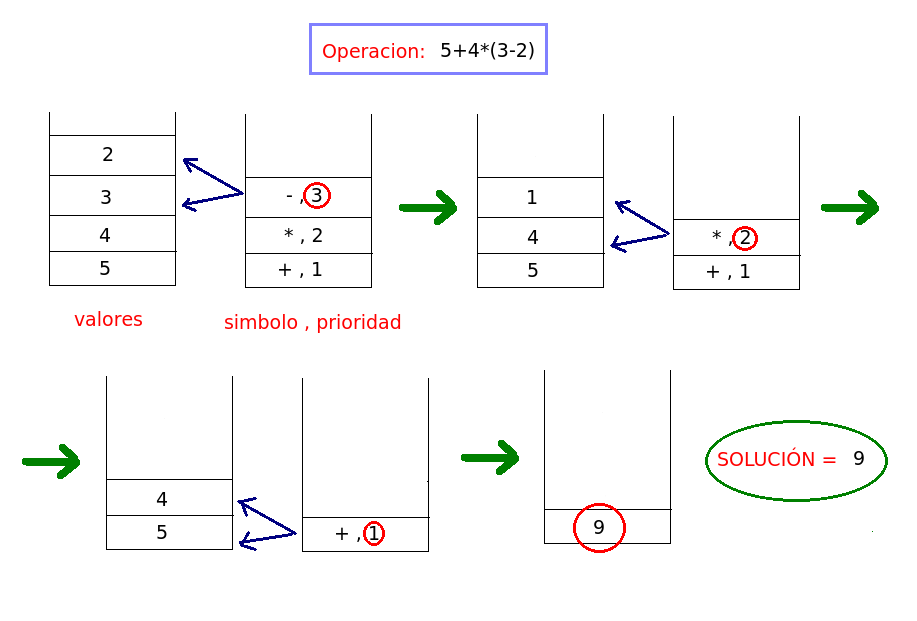
\includegraphics[width=0.8\textwidth,]{7.png}}%

\subsection{Restricciones de uso}
He de decir, que existen muchísimos casos problemáticos, los cuales habría que controlar para el correcto funcionamiento de la calculadora. 

Por mi parte he intentado crear las suficientes reglas que respalden a todos estos casos, pero es posible que no los haya abarcado todos, por lo 
que no me hago responsable del resultado de las operaciones o de la ejecución del programa, si no se cumplen \textbf{TODAS Y CADA UNA} 
de las restricciones siguientes:
\begin{enumerate}
    \item Para realizar cualquier operacion la sintaxis debe ser \textbf{[OPERACION] ?}.\newline\newline
    Ejemplos:
        \begin{enumerate}
            \item MAL:  (-5)*(3+4)\hspace{1cm}BIEN:  (-5)*(3+4) ?
            \item MAL:  (-55)\hspace{2.05cm}BIEN:  (-55) ?
            \item MAL:  a=a*b\hspace{1.75cm}BIEN:  a=a*b ?\newline 
        \end{enumerate}
       
	\item Los \textbf{numeros negativos} deben ir \textbf{siempre entre parentesis}.\newline\newline
    Ejemplos:
        \begin{enumerate}
            \item MAL:  -5*3 ?\hspace{1.5cm}BIEN:  (-5)*3 ?
            \item MAL:  -10 ?\hspace{1.75cm}BIEN:  (-10) ?
            \item MAL:  a=-5*3 ?\hspace{1cm}BIEN:  a=(-5)*3 ?\newline
        \end{enumerate}
    
    \item No debe existir \textbf{ningun espacio} en las operaciones.\newline\newline
    Ejemplos:
        \begin{enumerate}
            \item MAL:  (-5) * 3 ?\hspace{2.3cm}BIEN:  (-5)*3 ?
            \item MAL:  a = (-5) * 3 ?\hspace{1.5cm}BIEN:  a=(-5)*3 ?\newline
        \end{enumerate}

    \item Escribir \textbf{cualquier cosa} que no sea una operacion, una variable o una asignacion
    a una variable puede generar un \textbf{resultado inesperado}.\newline

    \item Puede utilizar un \textbf{número ilimitado de parentesis}, siempre y cuando no falte ninguno y respete 
    las restricciones anteriores.\newline

    \item No debe \textbf{dividir por cero}.\newline
\end{enumerate}

\textit{Nota: Es posible que algunas operaciones complejas con muchos parentesis y operadores devuelvan valores erroneos. 
No he sido capaz de solventar este problema, ya que ocurre solo en casos contados.}

\section{Compilación y modos de ejecución}
\subsection{Compilación}
Para compilar unicamente debemos ir a la carpeta donde se encuentra el fichero \textbf{calculadora.l}, abrir un terminal y ejecutar la orden \textbf{make}.
Esto generará un ejecutable llamado \textbf{calculadora}.

Para eliminar el ejecutable y los restos creados durante la compilación debemos ejecutar la orden \textbf{make clean} en un terminal.

\noindent\makebox[\textwidth][c]{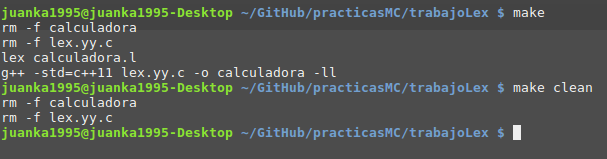
\includegraphics[width=0.7\textwidth,]{2.png}}%

\subsection{Modos de ejecución}
Tenemos dos formas de utilizar la calculadora, a través de \textbf{un fichero de texto} o de \textbf{la entrada manual de operaciones}.
\subsubsection{Fichero de texto}
Debemos de crear un fichero con las operaciones que deseamos que nuestra calculadora ejecute. Podemos basarnos en el fichero \textbf{entrada} que adjunto en el
interior del comprimido.

Seguidamente lanzamos la calculadora pasandole como parametro la ruta de dicho fichero de entrada.

\noindent\makebox[\textwidth][c]{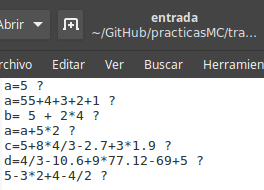
\includegraphics[width=0.3\textwidth,]{1.png}}%

\noindent\makebox[\textwidth][c]{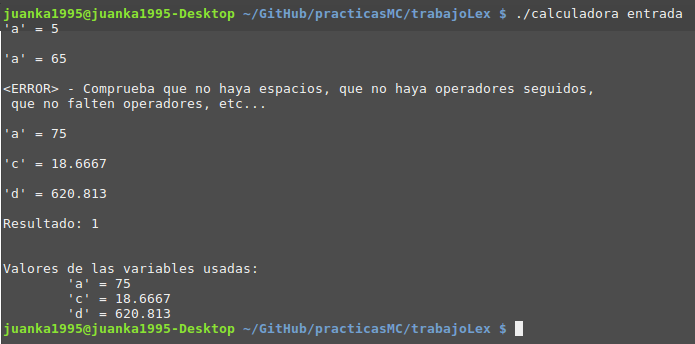
\includegraphics[width=0.7\textwidth,]{3.png}}%

\clearpage

\subsubsection{Entrada manual}
Simplemente deberemos ejecutar el programa y escribir las operaciones por teclado. Cuando terminemos deberemos pulsar la combinación \textbf{CTRL + D} para 
salir.

\noindent\makebox[\textwidth][c]{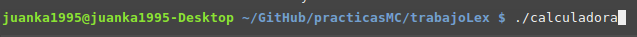
\includegraphics[width=0.7\textwidth,]{4.png}}%

\noindent\makebox[\textwidth][c]{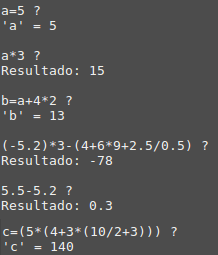
\includegraphics[width=0.25\textwidth,]{6.png}}%

\end{document}
